\section{Unified Virtual Addressing}
\label{sec-uva}

In this section, we talk about the Unified Virtual Addressing (UVA) feature that itegrates virtual memory spaces among GPUs and CPUs.
This technique allows not only bigger memory size, but also easy memory access among CPUs and GPUs.
We will talk about the concept of UVA, how we implemented UVA on Gluon, and finally discuss about the limitations and future
directions for better optimizations.

\subsection{UVA concept}
\begin{figure}
\centering
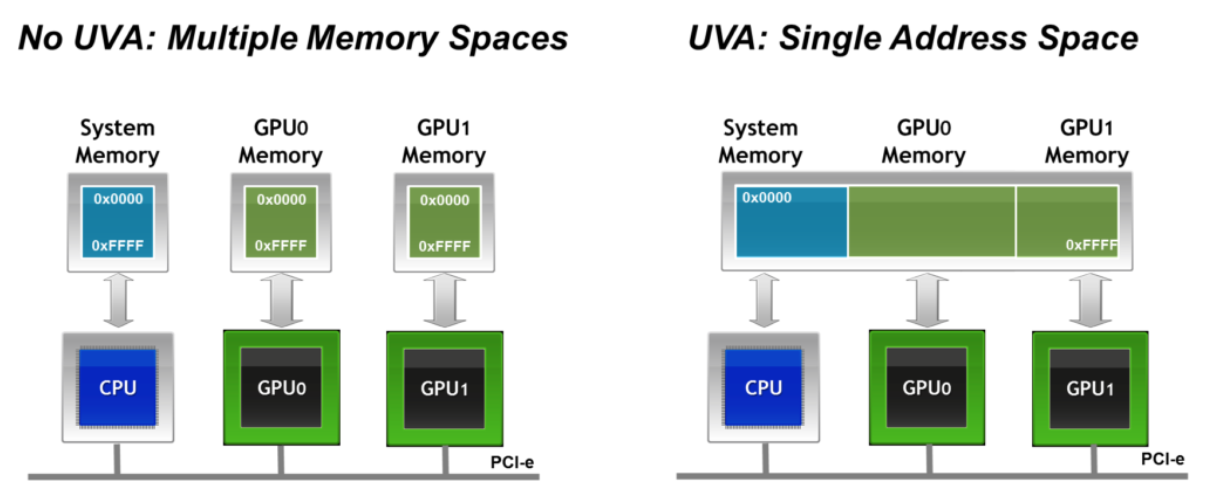
\includegraphics[width=0.49\textwidth]{uva-fig.png}
\mycaption{Unified Virtual Address}{The figure shows the address spaces with and without using UVA. 
}
\label{fig-uva}
%\vspace{-20pt}
\end{figure}

The GPU memory on servers is typically very limited.
So storing graphs in GPUs places a limitation on the size of the graph per node, requires larger clusters which increases communication overhead, 
and thus, could lose performance.
Furthermore, if the graphs are stored on the host memory, 
then the frequent data copy is required among hosts and devices memory since their address spaces are different.
These frequent data transfering overhead is expensive and makes implementations complicated. 


To avoid this cost of copying and storing large graph partitions per GPU separately,
NVIDIA introduced Unified Virtual Addresses (UVA). In UVA, both the GPU and the CPU memory lie in the same address space.
Therefore, the programmer does not need to worry about creating separate buffers for host memory and GPU memory. This is shown in Figure~\ref{fig-uva}. 

In UVA, memory is allocated in a region on the host using a call called cudaHostAlloc()~\cite{alloc-cuda}. This memory is pinned memory, and cannot be paged out by the virtual memory system. Once the memory is allocated, it can be accessed from CPU as well as GPU. Note that the access of this pinned memory from GPU can be done without any copying of data from host to GPU. GPU threads can directly access and process data located in the pinned memory on the host. This technique allows you to leverage host memory when your device has limited global memory and also allows you to explicitly transfer data between host and device. 

However, sharing zero-copy memory data between host and device involves synchronizing memory accesses across host and device, because modifying data in zero-copy memory simultaneously from host and device could lead to undefined behavior. 

\subsection{Using UVA in Gluon}
We applied UVA to the Gluon substrate. In the original Gluon implementation,
the node label data, as well as bitset and offset data are all presented in the device memory. 
Data including graph is partitioned across multiple devices, but still possible to invoke following issues due to 
the very limited memory: out-of-memory (OOM) or slow execution time due to exhaustive memory operations.
To alleviate these issues,
we utilized UVA to globally store graph, bitset, and offset data on the integrated memory space by using cudaHostAlloc().
Therefore, instead of using its memory, GPU can perform its computation on the shared memory with CPUs and other GPUs.
Moreover, the pinned memory allows to eliminations of the kernel interventions and fast execution time.

We tested our implementation on tuxedo server whose host memory size is 190GB, with 2 GPUs, each containing 8GB of device memory. 
In this environment, we potentially could expect 10x larger partitions than non-UVA host. 

\subsection{Discussion and Limitations}
We stored the entire data on the host memory using cudaHostAlloc(). Note that this leads to a non-trivial performance drop since all data has to be fetched from the host through the PCI interface, instead of accessing them through the fast bandwidth device memory.
There is a lot of opportunity to explore smarter strategies to place data on the shared memory like NUMA architecture.
For example, we can store some parts of the graph which might be cold regions that are not accessed frequently using UVA, and store the hot regions in device memory.
This would help us get not only memory operation time, but also extra capacity.

Newer GPUs also support a mode called Unified Memory, which is different from UVA;
The GPUs that we tested on does support for Unified Memory. 
In Unified Memory, the programmers get a similar interface as that of UVA with a single virtual address space for host and device memory.
However, unified memory leads to better performance by transferring data from the host to the device when the device needs it, and managing the synchronization with the host copy of the data transparently without any efforts by the programmer. This has potential to improve the performance significantly by using smart prefetching and readahead strategies to improve the locality of data, and also gain the high capacity of host memory. 
